\documentclass[10pt,letterpaper,onecolumn,draftclsnofoot]{IEEEtran}
\usepackage[margin=0.75in]{geometry}
\usepackage{listings}
\usepackage{color}
\usepackage{array}
\usepackage{booktabs}
\usepackage{hyperref}
\usepackage{enumitem}
%\usepackage{underscore}
\usepackage{graphicx}
\usepackage{float}
\usepackage{parskip}
\usepackage{courier}
\usepackage{pdfpages}
\definecolor{dkgreen}{rgb}{0,0.6,0}
\definecolor{gray}{rgb}{0.5,0.5,0.5}
\definecolor{mauve}{rgb}{0.58,0,0.82}

\hypersetup{colorlinks=true, linkcolor=black}

\lstset{frame=none,
  language=Python,
  columns=flexible,
  numberstyle=\tiny\color{gray},
  keywordstyle=\color{blue},
  commentstyle=\color{dkgreen},
  stringstyle=\color{mauve},
  breaklines=true,
  breakatwhitespace=true,
  tabsize=4
  %showstringspaces=false,
  %basicstyle=\ttfamily
}
\begin{document}
\begin{titlepage}
  \pagenumbering{gobble}
  \title{POWER8 Continuous Integration\\ Final Report}
  \author{Leon Leighton, Thomas Olson, Derek Wong\\Project 35}
  \date{June 13, 2017}
  \maketitle
  \vspace{4cm}
  \begin{abstract}
  \noindent This document contains an overview of the progress of the POWER8 Continuous Integration project.
    It includes the goals and purpose of the project, the current status, items remaining to be done, 
    and a discussion of problems we have encountered. 
 \end{abstract}
\end{titlepage}

\pagenumbering{arabic}
\setcounter{tocdepth}{2}
\tableofcontents
\clearpage
\section{Introduction}
IBM requested a project that would create an easy to use, public, Cloud-based, 
POWER8 Continuous Integration service in order to increase the ability
of Open Source projects to build and test their software on POWER8.
Open Source software projects are often designed to work on as broad a range of hardware architectures as possible. 
The users of Open Source software want the flexibility to consider a variety of hardware solutions in order to take advantage of different capabilities and to avoid vendor lock-in in the future. 
To support their users, Open Source software projects spend their time and resources on adding support for new architectures as they become available. 
The introduction of IBM's POWER8 architecture broadened the range of possible solutions available to the end users of Open Source software. 
This creates a need for Open Source projects to ensure that their software builds and functions correctly on POWER8. 
Open Source software projects often use Continuous Integration (CI) systems to build and test their software. 
CI enables these projects to validate their software after each change, ensuring that it continues to work as expected. 
Public Cloud-based solutions already exist to enable Open Source software developers to build and test their software on Intel's x86 architecture. 
Thus, while much of the work needed to enable software to compile on POWER8 has already been done at the compiler level, Open Source software developers still need an easy way to build and test their software on POWER8. \\

Our primary client at IBM was Gerrit Huizenga. Gerrit, along with Stan Gowen and
other IBM employees, took an active role in guiding the project while allowing us
to do the development. They provided us with the goals of the project and pointed
us to resources that were available for us to learn from. Toward the end of the
project they assisted us by providing test builds for the CI system. \\

The project team members were Leon Leighton, Thomas Olson, and Derek Wong. Leon
Leighton focused on OpenStack, Jenkins, and Ansible. Thomas Olson focused on build configuration and troubleshooting.
Derek Wong focused on deciding which plugins to use in Jenkins, such as the GitHub OAuth and the Build Notification Plugins. 

\section{Requirements Document}
\subsection{Introduction}
\subsubsection{Purpose}
The goal of this Software Requirements Specification is to set out the requirements for the POWER8 Build and Test Infrastructure project to help coordinate between the multiple stakeholders involved in bringing the project to fruition. This document is intended to be read by technically adept persons, with an emphasis on being read by the Oregon State University Open Source Lab, employees of IBM and faculty of the Oregon State University College of Engineering.
\subsubsection{Scope}
The POWER8 Build and Test Infrastructure shall automatically pull source code from online software repositories, build the required binaries for the POWER8 architecture, run required test suites on the binaries and make the binaries available for use. It shall allow interested parties to register their project's repository through an online interface to maximize ease of use. The system will vastly simplify the ability for open-source projects to test their source code on POWER8. This benefits the developers by allowing such projects to operate on a wider variety of platforms and benefits IBM by greatly increasing the accessibility of the POWER8 architecture to a enormous magnitude of open-source projects.
\subsubsection{Overview}
The rest of this Software Requirements Specification consists of the overall description of the system and the specific requirements for it as laid out in IEEE 830-1998, followed by the table of contents at the end of the document.

\subsection{Overall description}
\subsubsection{Product perspective}
The POWER8 Build and Test Infrastructure will interface with software code repositories such as GitHub to automatically pull source code from those repositories to be built. It will run natively on POWER8 architecture hosted by the Oregon State University Open Source Lab.
\subsubsection{Product functions}
The system will allow people to register projects hosted on GitHub through a web interface to be automatically built, tested and released. Once a project is registered, the system will pull the updated version of the source code for a given project when it is updated. It will build the binaries for the POWER8 architecture in either a VM or a container and test them with tests provided by the user for regressions and errors. The user will be notified if the build and/or test suites failed. If everything succeeds, the system will upload the tested and verified binaries such that the user may access them.
\subsubsection{User characteristics}
This system will be intended to be used by people interested in expanding the scope of what architectures are supported by their platform. It will be targeted towards open source software developers with some experience in building and releasing software.
\subsubsection{Apportioning of requirements}
The fundamental base-line goal is for the system to be able to automatically do a pull-build-deploy cycle for a given project. Once that is complete, adding a test step to the cycle and a web interface are the next two goals. If time permits, further stretch goals may be considered.

\subsection{Specific requirements}
\subsubsection{External interfaces}
\begin{enumerate}
\item GitHub repository
\item External authentication sources such as GitHub and Google.
\item Test suites
\item Test results
\item Produced binaries
\end{enumerate}
\subsubsection{Functional requirements}
\begin{enumerate}
\item The system shall allow people to register projects hosted on GitHub through a web interface
\item The system shall automatically build the software.
\item The system shall run tests specified by the project.
\item The system shall report the results of the test to the project.
\item The system shall make the resulting binaries available to the project.
\end{enumerate}
\subsubsection{Design constraints}
The software must compile and run on Linux running on POWER8.
\subsubsection{Software system attributes}
\paragraph{Security}
All project builds should be isolated from both the host system and other project builds.
\paragraph{Portability}
The CI system should be able to be run on other POWER8 systems with a minimal amount of configuration.

\section{Discussion of Requirements Document}
The requirements document is incomplete. In our discussions with IBM during the writing of this
document, they expressed that they wanted us to follow a more Agile style of developement to match
their internal use of Agile. As such, they did not want us to do an up front requirements document,
but rather focus on user stories as a basis of a design document. After speaking to Kevin McGrath
about these concerns he advised us to follow the direction from our client.

\clearpage
\section{Design Document}
\subsection{Introduction}
The goal of this document is to communicate the requirements and design of the POWER8 Continuous Integration project.
This information is conveyed in the form of user stories which contain three parts.
The `CARD' contains the requirement and the role of the stakeholder.
The `CONVERSATION' conveys how we intend to meet that requirement.
Finally, the `CONFIRMATION' indicates a way that the meeting of the requirement can be verified.
As can be seen from the user stories, the overall design of this project is one of integrating a number of existing resources and open source projects into a system which will provide a continuous integration system for IBM's POWER8 hardware.\\\\
Below is a list of the user stories and the author.\\

\begin{description}[leftmargin=12em,style=multiline]
  \item[POWER8 Cluster]
    POWER8 servers that can be used for Continuous Integration. Authored by Leon Leighton.\\
  \item[Deployment/Configuration Management]
    Manage installing the POWER8 CI system in a reproducible way. Authored by Leon Leighton.\\\\
  \item[Isolation]
    Isolate builds from each other and other users of the cluster. Authored by Leon Leighton.\\
  \item[Automation of VM and container creation/removal]
    Automate the creation and removal of virtual machines and containers. Authored by Leon Leighton.\\\\
  \item[Login]
    Use an existing login. Authored by Derek Wong.\\
  \item[Build Status]
    Informing user of build status. Authored by Derek Wong.\\
  \item[Persistant VMs]
    Persistent virtual machines for our website and Jenkins. Authored by Derek Wong.\\
  \item[Build Artifacts]
    Access the built and tested files. Authored by Thomas Olson.\\
  \item[Build/Environment Configuration]
    Configure the build and testing environment and methods. Authored by Thomas Olson.\\\\
  \item[Automation of Builds]
    Automatically run builds when a commit is made to the repository. Authored by Thomas Olson.\\
  \item[Pre-build VM images]
    The system should use pre-built images for the base system of VMs. Authored by Thomas Olson.\\
\end{description}


\subsection{User Stories}
\subsubsection{POWER8 Cluster}
\paragraph{CARD}
As an open source software developer, I want to build and test my software on POWER8, so that I can ensure proper functioning on that architecture.
\paragraph{CONVERSATION}
The goal of this project is to enable open source software projects to build and test their software on POWER8.
The OSU Open Source Lab has a POWER8 cluster that will serve as the hardware basis for this project.
The OSL POWER8 cluster runs OpenStack~\cite{openstackmain} and is managed via the Chef~\cite{chefmain} configuration management system.
We will be working closely with the OSL to ensure that we have access to the POWER8 cluster for both testing and deployment of our Continuous Integration system.
We will also work with the OSL to ensure that any needed OpenStack components are installed.
\paragraph{CONFIRMATION}
The POWER8 CI team members, in coordination with the OSL, are able to deploy the CI system on the OSL's POWER8 OpenStack cluster.

\subsubsection{Deployment/Configuration Management}
\paragraph{CARD}
As a system administrator, I want to centralize the management of the POWER8 CI system, so that there is a single source of truth for the configuration of the system.
\paragraph{CONVERSATION}
We will need to deploy and configure multiple components to create the POWER8 CI system.
In addition, one of the goals of our project is to enable others to recreate our POWER8 CI system.
We can meet these needs and goals by using a configuration management system.
Ansible~\cite{ansiblemain} is a IT automation solution that will allow us to manage the configuration and deployment of our CI system.
Specifically, we will be using Ansible playbooks to install and configure Jenkins and Jenkins plugins and any additional components of the CI system.
Also, we will be keeping the Ansible playbooks in version control to allow us to keep track of changes and rollback changes when necessary.
This will give us the flexibility we need to test changes while being able to return to a known good configuration.
\paragraph{CONFIRMATION}
Ansible playbooks exists that will deploy our CI system on a POWER8 OpenStack cluster.

\subsubsection{Isolation}
\paragraph{CARD}
As an open source software developer, I want my project builds to be isolated from other projects, so that my builds and test complete without outside interference.
\paragraph{CONVERSATION}
Our project will be hosted on the OSL's POWER8 OpenStack cluster and we want to ensure that our usage of the cluster does not negatively impact other users of the system.
Additionally, we do not want to run builds and tests in such a way that our users could interfere with each other.
We can achieve these ends by isolating builds and tests in virtual machines or Linux containers.
We will work with the OSL to determine appropriate quotas for usage of CPU, memory, and storage resources.
Our primary means of launching and removing virtual machines and containers will be through OpenStack's Nova and Magnum components.
By using these components we can leverage OpenStack's ability to manage virtual machines and Linux containers to provide isolation between different projects' builds and tests.
\paragraph{CONFIRMATION}
Projects are built in virtual machines or containers.
\subsubsection{Automation of VM and container creation/removal}
\paragraph{CARD}
As a system administrator, I want to automate the creation and removal of virtual machines and containers, so that projects are not waiting on manual intervention.
\paragraph{CONVERSATION}
The primary goal of this project is to provide an automated solution for open source projects to build and test their software on POWER8.
To meet this goal we will need to have the ability to automate the creation and removal of the virtual machines and containers where the builds will take place.
As mentioned in another user story, OpenStack has the ability to manage virtual machines and containers through the Nova and Magnum components.
In order to automate this, we will utilize Jenkins~\cite{jenkinsmain} which has the ability to interact with OpenStack by using a plugin~\cite{jcloudsplugin}.
This will give us the ability to automate the creation and removal of VMs and containers.
\paragraph{CONFIRMATION}
The creation and removal of the virtual machines and containers used for building and testing is automated.

\subsubsection{Login}
\paragraph{CARD}
As an open source software developer, I want to be able to use an existing login, so that I don't have to create another account.
\paragraph{CONVERSATION}
We will use pluggable authentication from Jenkins. The plugins will allow user to use login credentials from other web sites, such as GitHub~\cite{githublogin}, Google~\cite{googlelogin}, etc\ldots to login. The plugins can simply be installed through Jenkins.
\paragraph{CONFIRMATION}
Our registration web site will allow developers to choose from multiple options for authentication when registering.

\subsubsection{Build Status}
\paragraph{CARD}
As an open source software developer, I want to see my build status, so I know if my build passed or failed.
\paragraph{CONVERSATION}
We will use a plugin from Jenkins to display the status of our developer's build. More specifically, we intend to use the Build Monitor Plugin~\cite{buildmonitor} to display the information to our users. The Build Monitor Plugin supports many features such as: display the status and progress of selected jobs, display the names of people who might be responsible for `breaking the build', display who is fixing a broken build, and display what broke the build. The plugin can be installed through Jenkins.
\paragraph{CONFIRMATION}
Our web site will allow developers to see their build status (pass/fail).

\subsubsection{Persistent VMs}
\paragraph{CARD}
As a system administrator, I want persistent virtual machines (VMs) for our website and Jenkins, so that I have a platform to host my service.
\paragraph{CONVERSATION}
We will use OpenStack to deploy our virtual machines. Then we will use those virtual machines to host our website and Jenkins. OpenStack is a set of software tools for building and managing cloud computing platforms, more specifically it is used to deploy virtual machines to handle different tasks. For our website, we will be using Apache HTTP Server.
\paragraph{CONFIRMATION}
Our website and Jenkins will be hosted on virtual machines.

\subsubsection{Build Artifacts}
\paragraph{CARD}
As an open source software developer, I want to access the built and tested files, so that I can distribute them to users.
\paragraph{CONVERSATION}
Developers need to be able to access the created binaries and other files from building the source code, so that they may
be able to distribute them as needed on their own.
\paragraph{CONFIRMATION}
The files can be downloaded from the website.

\subsubsection{Build/Environment Configuration}
\paragraph{CARD}
As an open source software developer, I want to configure the build and testing environment and methods, so that I can be sure it matches my standard build process.
\paragraph{CONVERSATION}
Each repository needs a way to configure things such as required packages for building and command-line arguments.
To that end, the system will require a configuration file in YAML format. This file will contain information such as necessary
libraries and packages, programs and command-line arguments for building, and how to test the built code.
\paragraph{CONFIRMATION}
The system checks for a file called '.powerci.yml' in registered repositories and configures the build environment with it.

\subsubsection{Automation of Builds}
\paragraph{CARD}
As an open source software developer, I want the system to automatically run builds when a commit is made to the repository, so that I can determine if a bug has been introduced as early as possible.
\paragraph{CONVERSATION}
Developers require a system that will automatically pull, build and test so they can always have the most current
binaries available and so they can quickly know if a recent change causes the build to fail. Jenkins has plugin support for polling
Git repositories for changes and then executing a pull-build-test-deploy sequence when a commit is detected to have been pushed since
the last build was ran.
\paragraph{CONFIRMATION}
The system automatically executes a pull-build-test-deploy sequence when a commit is pushed to the Git repository.

\subsubsection{Pre-build VM images}
\paragraph{CARD}
As an open source software developer, I want to be able to choose from pre-built virtual machine, so that my builds and tests can target a known platform. 
\paragraph{CONVERSATION}
Pre-built images that are used for spinning up VMs makes the entire process of deploying and configuring a VM
for running a pull-build-test sequence much faster and smoother. Ubuntu will probably be the OS of choice for the base images, however
we may look into providing images for other Linux distributions.
\paragraph{CONFIRMATION}
The system uses disk images with Linux installed for starting VMs.

\section{Updates to Design Document}
\subsection{Login}
Updated the "Login" user story. Originally, we planned to let users use their existing credentials from different websites such as GitHub, Google, etc, but we narrowed it down to just GitHub for now. Allowing them to use other accounts will be more of a stretch goal in the future. The following is the updated user story.
\subsubsection{CARD}
As an open source software developer, I want to be able to use my github account credentials to login, so that I don't have to create another account, to access Jenkins.
\subsubsection{CONVERSATION}
We will use pluggable authentication from Jenkins to accomplish this task. Specifically, we will use the GitHub OAuth Plugin to allow users to login with their GitHub credentials.
\subsubsection{CONFIRMATION}
Our registration web site will allow developers to simply use their GitHub credentials to login into our services.
\subsection{Resource Management}
Replaced "Automation of VM/container creation/removal" card with "Resource Management" card in order to capture the reasoning behind automating creation/removal of build resources. The following is the updated user story.
\subsubsection{CARD}
As an open source software developer, I want my project builds to finish in a timely manner, so that I can receive build and test feedback as quickly as possible.
\subsubsection{CONVERSATION}
The users of our project want their builds to run as soon as possible.
However, our project has a finite amount of resources available on the POWER8 OpenStack cluster.
This may cause a delay in starting a build if the necessary resources are not available.
Builds should be queued to run in the order received if the resources are not available to run them immediately.
In order to ensure that resources are available for new builds, we will need to automatically remove old VMs and containers.
As mentioned in another user story, OpenStack has the ability to manage virtual machines and containers through the Nova and Magnum components.
In order to automate this, we will utilize Jenkins~\cite{jenkinsmain} which has the ability to interact with OpenStack by using a plugin~\cite{jcloudsplugin}.
This will give us the ability to automate both the creation and removal of VMs and containers.
\subsubsection{CONFIRMATION}
Builds are triggered immediately if resources are available, and queued in the order recieved otherwise.
\clearpage
\section{Tech Review Document}
\subsection{Introduction}
This document contains an evaluation of nine pieces of technology that we will be using in the IBM POWER8 Continuous Integration project.
We define evaluation criteria based on the goal we are attempting to achieve by using that piece.
For each piece we have selected three options, and we choose the best option based on the evaluation.\\\\
The nine pieces are:\\
\begin{description}[leftmargin=12em,style=multiline]
  \item[Cluster Management]
    The software that will be used to manage a cluster of POWER8 nodes. Authored by Leon Leighton.\\
  \item[Continuous Integration Software]
    The software that will perform the building and testing of projects. Authored by Leon Leighton.\\\\
  \item[Configuration Management]
    System that will be used to manage the configuration of the system. Authored by Leon Leighton.\\\\
  \item[Linux Distribution Support]
    The Linux distribution that projects will be built and tested on. Authored by Thomas Olson.\\\\
  \item[Platform For Running Builds]
    The type of platform used for building and testing. Authored by Thomas Olson.\\\\
  \item[Configuration File Format]
    The file format that will be used by projects for configuring builds. Authored by Thomas Olson.\\\\
  \item[Login/Authentication]
    Method for users to login to the system. Authored by Derek Wong.\\\\
  \item[Frontend/Web Frameworks]
    Method of creating a user interface for interacting with the system. Authored by Derek Wong.\\\\
  \item[Tracing State of Builds/Tests]
    Functionality to show users the status of their builds and tests. Authored by Derek Wong.\\\\
\end{description}
\subsection{Cluster Management}
\subsubsection{Options}
\paragraph{OpenStack}
OpenStack~\cite{openstackmain} is a cluster management solution originally created by Rackspace and NASA, and now managed by the OpenStack Foundation.
It contains a number of projects that provide services such as object and block storage, identity management, networking and compute resource management, bare metal provisioning, and DNS services~\cite{openstackservices}.
This modular approach allows users to select which parts they need to accomplish their goals without having to install components they will not be using.
\paragraph{CloudStack}
CloudStack~\cite{cloudstackmain} is an Apache Software Foundation cluster management project which aims to provide many of the same services as OpenStack.
It follows a more monolithic approach where most components are distributed as part of a single binary~\cite{cloudstackmono}.
\paragraph{Ganeti}
Ganeti~\cite{ganetimain} is a cluster management solution from Google that focuses on managing virtual machines.
It can be used to create new virtual machines, manage disks, and manage failover of virtual machine instance.
\subsubsection{Goals for use}
The primary goal for using cluster management software is to manage the creation and destruction of temporary virtual machines and containers that will be used for building and testing projects.
\subsubsection{Criteria for Evaluation}
\begin{enumerate}
  \item Community Support: Our chosen solution should have a community that provides support in the form of documentation, bug fixes, and assistance.
  \item Linux Support: Linux must be supported as both host and guest.
  \item Container Support: Optional, but we would like to have support for building and testing in containers.
  \item Jenkins Plugin Support: Jenkins is a likely piece of our solution, therefore having a Jenkins plugin that interacts with our cluster management solution is highly desired.
\end{enumerate}
\subsubsection{Table}
\begin{center}
  \begin{tabular}{llll}
    Criteria & OpenStack & CloudStack & Ganeti \\ \midrule
    Community Support       & Yes & Yes & Yes \\ \midrule
    Linux Support           & Yes & Yes & Yes \\ \midrule
    Container Support       & Yes & Partial & No \\ \midrule
    Jenkins Plugin Support  & Yes & Yes & No \\ \bottomrule
  \end{tabular}
\end{center}
\subsubsection{Discussion}
OpenStack, CloudStack, and Ganeti can all run on Linux and can host Linux virtual machines.
Ganeti does little more than this, however, and will not be considered further.
Both OpenStack and CloudStack can interact with Jenkins through a plugin~\cite{jcloudsplugin}~\cite{jcloudsproviders}.
OpenStack appears to have a larger community and a more mature container solution than CloudStack.
\subsubsection{Selection of best option}
OpenStack is our chosen solution for cluster management. It meets all of our criteria for evaluation.

\subsection{Continuous Integration Software}
\subsubsection{Options}
\paragraph{Jenkins}
Jenkins~\cite{jenkinsmain} is an automation server that can be used to automate builds, tests, and deployments.
It is extensible and has a large number of plugins that enable it to interact with other systems. 
\paragraph{Buildbot}
Buildbot~\cite{buildbotmain} is another system that enables the automation of builds, tests, and deployments.
It can be extended through the use of Python configuration files~\cite{buildbotconfig}. 
\paragraph{Strider}
Strider~\cite{stridermain} is a continuous integration server written in Node.js.
Like Jenkins it uses plugins to extend its functionality.
\subsubsection{Goals for use}
Automate building and testing Open Source projects.
\subsubsection{Criteria for Evaluation}
\begin{enumerate}
  \item Open Source: As our target audience is Open Source software developers, we should use an Open Source solution to be consistent with the community.
  \item Language Support: We need to be able to build and test projects written in a variety of languages.
  \item Notifications: We need some way of providing the user with feedback on the status of their builds and tests.
  \item Extensible: If we find that there are missing features we will need some way of extending the functionality of the software.
  \item Number of Existing Plugins: A larger number of plugins increases the probability that someone may have already provided functionality that we need that is not already in the software.
\end{enumerate}
\subsubsection{Table}
\begin{center}
  \begin{tabular}{llll}
    Criteria & Jenkins & Buildbot & Strider \\ \midrule
    Open Source       & Yes & Yes & Yes \\ \midrule
    Language Support  & Any & Any & Any \\ \midrule
    Notifications     & Yes & Yes & Yes \\ \midrule
    Extensible        & Yes & Yes & Yes \\ \midrule
    Number of Plugins & High & Low & Medium \\ \bottomrule
  \end{tabular}
\end{center}
\subsubsection{Discussion}
All three of our options meet our basic evaluation criteria.
However, there is quite a large difference in the number of plugins available, with Jenkins~\cite{jenkinsplugins} having a much larger number than Buildbot~\cite{buildbotplugins} or Strider~\cite{striderplugins}.
There is also a large variety in the type of plugins for Jenkins, covering functionality such as source code management, reports and notifications, and UI elements~\cite{jenkinsplugins}.
\subsubsection{Selection of best option}
With its large number and variety of plugins, Jenkins is our chosen solution for continuous integration software.

\subsection{Configuration Management}
\subsubsection{Options}
\paragraph{Ansible}
Ansible~\cite{ansiblemain} is a configuration management and infrastructure automation solution.
It is agentless, using SSH to connect to and run commands on nodes.
Ansible uses YAML files for configuration~\cite{ansibleworks}.
\paragraph{Chef}
Chef~\cite{chefmain} is a configuration management solution that uses agents running on each node to poll a central server to access configuration `cookbooks' that are written in Ruby~\cite{chefworks}.
\paragraph{Puppet}
Puppet~\cite{puppetmain} is also a configuration management solution.
Like Chef, it uses agents on each node and a central `puppet master' server~\cite{puppetworks}.
Configuration is done in a language specific to Puppet that is meant to be accessible to system administrators~\cite{puppetlang}.
\subsubsection{Goals for use}
Using a configuration management system will allow us to create a solution that can be replicated by others who may wish to setup their own POWER8 Continuous Integration system.
Used in conjunction with a version control system, it will also give us the ability to roll back changes that have been made, giving us flexibility in experimenting with different options as we progress through the project. 
At a higher level, a configuration management system will allow us to specify what we want the state of the system to be, and it will also give us an ultimate `source of truth' for the project.
\subsubsection{Criteria for Evaluation}
\begin{enumerate}
  \item Support for installing Jenkins: Our chosen solution should have the ability to manage our Continuous Integration software. 
  \item Overhead: Like most projects, we wish to reduce the amount of overhead in our system.
  \item Difficulty: We should choose simpler solutions when possible.
\end{enumerate}
\subsubsection{Table}
\begin{center}
  \begin{tabular}{llll}
    Criteria & Ansible & Chef & Puppet \\ \midrule
    Installs Jenkins       & Yes & Yes & Yes \\ \midrule
    Overhead           & Low & Moderate & Moderate \\ \midrule
    Difficulty           & Low & Moderate & Moderate \\ \bottomrule
  \end{tabular}
\end{center}
\subsubsection{Discussion}
As we are likely to use Jenkins for our continuous integration software we would like there to be an already existing method to install and configure it with the option we choose for configuration management.
All three options under consideration meet this criteria through user created modules.
We would also like to reduce the overhead involved in using a configuration management system.
Both Puppet and Chef require the use of a master server and an agent installed on any node that will be managed.
While this is not a high level of overhead, we do contrast that with Ansible which uses SSH which is already included on most Linux systems.
It should be noted, however, that since Ansible uses SSH, we will need to create and secure the SSH keys that will be used for authentication.
Ansible is also noted to be easier to setup and use.~\cite{cmcompare}
\subsubsection{Selection of best option}
While all three options would allow us to accomplish our goals, we have selected Ansible as our best option.

\subsection{Linux Distribution Support}
\subsubsection{Options}
\paragraph{RedHat Enterprise Linux}
RedHat Enterprise Linux is widely considered to be one of the standard Linux distributions for server environments, having been around for a number of years and being very stable. It is supported by the Red Hat corporation and has a ten-year supported production cycle for each major version, followed by an extended support period\cite{rhlife}. Unlike most Linux distributions, it has a paid subscription requirement for support and the extended support has a higher price. However, as a paid product, Red Hat provides dedicated support and certifications which can be important if such certifications are required for a project or if the project requires high availability and dedicated support in case issues arise.
\paragraph{CentOS}
CentOS is an unbranded version of RedHat Enterprise Linux, providing the same functionality and stability with only very minor functional differences. It is supported by the CentOS Project and is free for all use. As a result, it does not have the certifications nor the dedicated support of RedHat Enterprise Linux. As it tries to track the development of RedHat Enterprise Linux very closely, CentOS has approximately the same ten-year support cycle\cite{centlife}, but it does not have the same extended support period provided by Red Hat.
\paragraph{Ubuntu Server}
Ubuntu Server is a version of the Ubuntu distribution that differs from the desktop version only by the installer and the life cycle\cite{ubuntulife}. It is supported by Canonical and has a five-year life cycle per major version. Like CentOS, it is free to use, but Canonical optionally offers a contract for dedicated support. Ubuntu also tends to update application packages sooner, trading some amount of stability for newer functionality.
\subsubsection{Goals for use}
The operating system  selection will have a major effect on the stability and ease-of-use of the entire system. Our goal is to select an operating system that is stable, widely supported and easy to work with.
\subsubsection{Criteria for Evaluation}
\begin{enumerate}
  \item Stability: It is important that the operating system used for running builds has as few issues as possible so as to minimize the need for manual intervention in case there's a failure.
  \item Support: The operating system should have a strong support base to maximize ease of maintenance and help ensure longevity.
  \item Usability: The greater the usability and ease of configuration, the easier it becomes to maintain and improve the reliability of the system.
  \item Cost: The less the entire system costs, the better.
\end{enumerate}
\subsubsection{Table}
\begin{center}
  \begin{tabular}{llll}
    Criteria & RedHat & CentOS & Ubuntu Server \\ \midrule
    Stability       & Highest & High & Moderate \\ \midrule
    Support           & Highest & Moderate & Moderate \\ \midrule
    Usability       & High & High & High \\ \midrule
    Cost       & High & None & None \\ \bottomrule
  \end{tabular}
\end{center}
\subsubsection{Discussion}
As this project does not require high availability or dedicated support, the benefits of buying a subscription for Red Hat Enterprise Linux are negligible, especially being that CentOS has much of the same functionality and the same length support cycle. This project also does not require an operating system that provides newer functionalities sooner like Ubuntu does, stability being a more important requirement.
\subsubsection{Selection of best option}
We have opted for using CentOS as the operating system that builds will be ran on and tested against. It provides the necessary stability and a wide base of support with a ten-year life cycle, while also being easy to configure, deploy and maintain.
\subsection{Platform for Running Builds}
\subsubsection{Options}
\paragraph{Virtual Machine}
Virtual Machines perform hardware-level emulation and do not allow the guests any access to the underlying operating system or hardware. They're the standard for situations where multiple OS's need to be deployed. Because they emulate all the hardware, there's nearly no risk of a malicious guest system affecting the host system. However, running a virtual machine requires a full operating system to be installed on each individual instance, causing them to take up a relatively significant amount of space per virtual machine compared to to size of the applications running on them. Additionally, their performance suffers due to having to emulate assembly-level instructions instead of executing them directly.
\paragraph{Container}
Containers perform operating system virtualization, allowing for multiple independent user-spaces to exist at the same time. Because they emulate parts of the operating system and not the physical hardware hardware, containers still need to allow some level of direct hardware access for applications to run properly. They also use some libraries provided by the host operating system instead of providing their own. As a result, they tend to be much smaller than a full-fledged virtual machine and run somewhat faster. A relatively new technology compared to virtual machines, they're rapidly gaining popularity in situations where hardware emulation is not required and restricting access to the host operating system is not a concern.
\paragraph{Bare metal}
Bare metal servers would have no virtualization or emulation; builds and tests would be ran directly on the hardware itself. The benefits of bare metal are speed and security; no emulation layer exists between the applications and the hardware and there is no host operating system for a malicious guest to interfere with. Builds would also be unable to hoard system resources, preventing a situation where one build slows down another. The single major downside is the requirement for a full physical server per each build that would be ran, greatly restricting the ability for multiple builds to be ran in parallel
\subsubsection{Goals for use}
The goal of selecting the platform the builds would interact with is to allow builds a host system to be ran and tested on while providing reliability and security for the underlying system.
\subsubsection{Criteria for Evaluation}
\begin{enumerate}
  \item Scalability: Ideally, it should be easy to scale the system up to allow a large number of simultaneous builds.
  \item Performance: Our selection should not significantly decrease the performance of the build-test process.
  \item Security: Being that we will compiling and testing untrusted and unverified code, it is important for the selected platform to minimize the ability of the build to negatively affect the host.
  \item Reliability: It is preferable that one build does not use up so many resources as to significantly reduce the speed of other builds being ran.
\end{enumerate}
\subsubsection{Table}
\begin{center}
  \begin{tabular}{llll}
    Criteria & Virtual Machines & Containers & Bare metal \\ \midrule
    Scalability       & High & Highest & Low \\ \midrule
    Performance           & Moderate & High & Highest \\ \midrule
    Security       & High & Moderate & Highest \\ \midrule
    Reliability  & High & High & Highest \\ \bottomrule
  \end{tabular}
\end{center}
\subsubsection{Discussion}
Although bare metal servers have undeniably the best performance, security and reliability, they simply do not have the scalability required for a project like this. Depending on storage space and resources, virtual machines and containers could potentially run upwards of one hundred builds simultaneously on a single server, negating the performance benefits. Furthermore, virtual machines provide nearly the same level of security and safety that a bare metal server provides, while containers can nearly match them in terms of performance.

Between virtual machines and containers, virtual machines provide better security and have years of support behind them, while containers provide better performance; virtual machines can have a performance penalty upwards of ten percent due to overhead.\cite{RC25482} Both virtual machines and containers allow for limiting the resources provided to a running instance, meeting the reliability requirements. They are also both exceedingly easy to configure for automated deployment, making them highly scalable.
\subsubsection{Selection of best option}
Although virtual machines can have a noticeable performance penalty due to overhead, this can be reduced with proper tuning. Furthermore, we believe that the better isolation and security provided by virtual machines can easily outweigh the performance penalties. Therefore, we have decided that virtual machines are the ideal platform for running the builds and tests on.

\subsection{Configuration File Formats}
\subsubsection{Options}
\paragraph{YAML}
YAML is a data-oriented markup language that is very concise while still being highly expressive. Notably, Ansible already uses YAML for its configuration files.
\paragraph{JSON}
JSON is a data-interchange format that is very concise, focused around key-value pairs. Its readability can suffer at times due to being designed with automated usage in mind instead of being human-generated.
\paragraph{XML}
XML is a document markup language that is incredibly powerful and expressive. However, it tends to being excessively verbose, making it somewhat difficult to read.
\subsubsection{Goals for use}
The configuration file will be included in a Git repository and will be how the system determines builds and tests are ran and interpreted. It should use a format powerful enough to accurately express all the information that the system will require without being unnecessarily complicated.
\subsubsection{Criteria for Evaluation}
\begin{enumerate}
  \item Expressiveness: The file format needs to be able to sufficiently express the users needs for building and testing their project.
  \item Readability: The ideal file format will be easy for a user to create and modify to suit the needs of their project.
\end{enumerate}
\subsubsection{Table}
\begin{center}
  \begin{tabular}{llll}
    Criteria & YAML & JSON & XML \\ \midrule
    Expressiveness       & High & Moderate & Highest \\ \midrule
    Readability       & Highest & High & Moderate \\ \bottomrule
  \end{tabular}
\end{center}
\subsubsection{Discussion}
XML is the most expressive of the three options, but it is unlikely we would need the power provided by it. JSON is on the opposing end of the spectrum, being so simple that it might not be powerful enough for what we need. In the middle lies YAML, powerful and highly readable due to it conciseness. Aditionally, Anisble using YAML gives YAML the bonus of already being used in this project.
\subsubsection{Selection of best option}
We have selected YAML as the file format for configuration files due to it being powerful, concise and consistent with what Ansible uses.

\subsection{Login/Authentication}
\subsubsection{Options}
\paragraph{GitHub Login Plugin}
The GitHub Login Plugin uses a github account for authentication.
\paragraph{Active Directory Plugin}
The Active Directory Plugin is a plugin for Jenkins and it uses Active Directory to authenticate the username and password.
\paragraph{Jenkins Login}
The Jenkins login is simply a Jenkins account and users are able to create it on the Jenkins website.
\subsubsection{Goals for use}
The goal for having an authentication is to provide our users a safe and secure place to build their project and to use our continuous integration service.
It will help prevent hackers from obtaining private information that could be detrimental to our users.
This is a security measure that is absolutely necessary for our project.
\subsubsection{Criteria for Evaluation}
\begin{enumerate}
  \item Security: Security is what keeps users confidential information such as source code from being leaked.
\end{enumerate}
\subsubsection{Table}
\begin{center}
  \begin{tabular}{llll}
    Criteria & GitHub Login Plugin & Active Directory Plugin & Jenkins Login\\ \midrule
    Security       & Yes & Yes & Yes \\ \midrule
  \end{tabular}
\end{center}
\subsubsection{Discussion}
The github login plugin is a really straight forward method for authentication.
Users can simply use their github accounts to login.
The second option is to use the active directory plugin.
This plugin is used with Jenkins to authenticate the username and password through active directory~\cite{activedirectory}.
The third option is to use Jenkins’ login.
Users can simply create a Jenkins’ account and have access to its functionalities.
They will also have the ability to give authorizations to different accounts for their projects.
\subsubsection{Selection of best option}
The best option is to use GitHub login plugin.
Most of our users will be using github for their projects, so it is most resonable to use the github login plugin for authentication.

\subsection{Frontend/Web frameworks}
\subsubsection{Options}
\paragraph{Tomcat}
Tomcat is an open source implementation of Java Servlet, JavaServer Pages, Java Expression Language and Java WebSocket technologies. 
\paragraph{Glassfish}
GlassFish is an open source application server; more specifically it is for the Java EE platform (Java Enterprise Edition).
\paragraph{Jetty}
Jetty provides a Web server and javax.servlet container, and it supports many components such as HTTP/2, WebSocket, OSGi (Open Service Gateway Initiative), JMX (Java Management Extensions), JNDI (Java Naming and Directory Interface), JAAS (Java Authentication and Authorization Service) and many other integrations.
\subsubsection{Goals for use}
The goal for having a web framework is so that our users have a platform to use our continuous integration service.
We will provide a simple and easy to use user interface (UI) so that our users would not have a complicated time using our services.
\subsubsection{Criteria for Evaluation}
\begin{enumerate}
  \item Usability: Having an easy-to-use user interface can give our users an easier time to use our service and it will help reduce confusion.
  \item Security: Security is important for our web framework because we don't want hackers to gain access to our services and obtain confidential information.
  \item Stability: Stability is needed because our service need to maintain at a functional state at all time so that it doesn't hinder our users from working
  \item Load time: The page load time should load at a reasonable speed so that our users would not have to wait a long time using our service.
\end{enumerate}
\subsubsection{Table}
\begin{center}
  \begin{tabular}{llll}
    Criteria & Tomcat & Glassfish & Jetty \\ \midrule
    Usability       & High & High & Moderate \\ \midrule
    Security           & Moderate & High & High \\ \midrule
    Stability      & Highest & High & High \\ \midrule
    Load time  & High & High & High \\ \bottomrule
  \end{tabular}
\end{center}
\subsubsection{Discussion}
Tomcat is very popular and it is known as a lightweight application that offers all the basic features required running a server.
It is an open source project so it is cost free.
It is highly flexible because it allows users to tweak their code as they see fit, and it has many built-in features~\cite{tomcat}.
The second option is Glassfish and it is also an open source project, which means that it is free of cost.
It has high performance and it was considered the fastest open source application server, according to SPECjAppServer2004 benchmark results~\cite{glassfish}.
Jetty provides a Web server and javax.servlet container.
They have a heavy focus on multi-connection HTTP and features such as SPYDY, which can significantly reduce page load latencies~\cite{jetty}.
\subsubsection{Selection of best option}
Overall, all three of the options are great, but the best option to use is Tomcat.
Glassfish has a lot of features and is the biggest out of the three options, but we are only using it for our frontend, so most features are unnecessary.
It has a big memory footprint, which means that it would consume more resources.
Jetty is a very light application and it consumes the least amount of resources but it is too small for our project.
Tomcat is ideal because it sits in between these two options and it offers a good amount of features to use.

\subsection{Tracing State of builds/tests}
\subsubsection{Options}
\paragraph{Build Monitor Plugin}
The Build Monitor Plugin is a plugin in Jenkins that provides a detailed view of the status of selected Jenkins jobs.
\paragraph{Lava Lamp Notifier}
The Lava Lamp Notifier is a notifier that indicate job status using a Lava Lamp.
\paragraph{Radiator View Plugin}
The Radiator View Plugin is a plugin in Jenkins and Hudson that provides a job view, which displays project status.
\subsubsection{Goals for use}
The goal to having the functionality to trace the build and test state is so that our users can see the status of their projects.
This will reveal the success or failure of projects that were build by our service and it will show where the failures have occurred.
\subsubsection{Criteria for Evaluation}
\begin{enumerate}
  \item Usability: Having an easy-to-use user interface (UI) allows our users to operate our service with minimal issues.
  \item Feature to display pass or fail builds:The ability to display pass or fail build is  the main purpose for this technology so this is a must have
  \item Feature to display progress of builds: The feature to display progress when building a project is helpful for our users to see how much longer it will take until their build is complete
  \item Feature to display where an error has occurred for build fails: The feature to see where an error has occurred in the build process is another important criteria; it will help developers ave time from manually tracking down the problem.
\end{enumerate}
\subsubsection{Table}
\begin{center}
  \begin{tabular}{llll}
    Criteria & Build Monitor Plugin & Lava Lamp Notifier & Radiator View Plugin \\ \midrule
    Usability       & Yes & None & Yes \\ \midrule
    Display pass or fail builds           & Yes & Yes & Yes \\ \midrule
    Display progress of builds       & Yes & None & None \\ \midrule
    Display where an error has occurred if build fails  & Yes & None & None \\ \bottomrule
  \end{tabular}
\end{center}
\subsubsection{Discussion}
The build monitor plugin supports many features and incorporates other plugins as well.
The features in this plugin include:
\begin{itemize}
  \item Displays the status and progress of selected jobs, the view is updated automatically every couple of seconds using AJAX\@. No `Enable Auto Refresh' needed.
  \item Displays the names of people who might be responsible for `breaking the build'.
  \item Supports the Claim plugin, so that you can see who's fixing a broken build.
  \item Supports View Job Filters, so that you can easily create Build Monitors for `slow builds', `only failing', etc.
  \item Supports Build Failure Analyzer, so that you know not only who, but also what broke the build.
  \item Supports CloudBees Folders Plugin, so that you can have project- and team-specific nested Build Monitors.
  \item The number of columns and size of the font used is easily customizable, making it trivial to accommodate screens of different sizes.
  \item UI configuration is stored in a cookie, making it possible to display different number of columns and using different font size on each of the screens at your office.
  \item Can work in a colour-blind-friendly mode
  \item~\cite{buildmonitor}
\end{itemize}
The lava lamp notifier is a really simple design created to indicate if a build passed or fail.
The only necessary component to use this type of method to track our build status is a USB LED light.
The light will simply light up green for pass and red for fail~\cite{lavalamp}.
This is not ideal for our type of project because our users would like to know more information than just a pass or fail notification.
The third option is the radiator view plugin.
This plugin is somewhat similar to the build monitor plugin but with less features.
It will display all the project that are building and indicate pass or fails on screen~\cite{radiatorview}.
\subsubsection{Selection of best option}
The best option to use is the build monitor plugin.
This technology has the most features out of all the other options I listed, and all the features are very useful for our users.

\subsection{Conclusion}
The following is a summary of the choices we have made for the nine pieces that we have evaluated.\\
\begin{enumerate}
  \item Cluster Management: OpenStack
  \item Continuous Integration Software: Jenkins
  \item Configuration Management: Ansible
  \item Linux Distribution Support: CentOS
  \item Platform For Running Builds: Virtual Machines
  \item Configuration File Format: YAML
  \item Login/Authentication: GitHub Login Plugin
  \item Frontend/Web Frameworks: Tomcat
  \item Tracing State of Builds/Tests: Build Monitor Plugin
\end{enumerate}
\section{Updates to Tech Review Document}
One minor point of revision for the Tech Review Document involved fixing an error in the Login/Authentication section.
The GitHub login plugin was supposed to be GitHub OAuth plugin and that is the plugin that we implemented in Jenkins.  

Two larger changes for our Tech Review was a change to the OS selection to indicate the client's desire that we use Ubuntu
and the platform selection to indicate the client's desire that we also support containers along with virtual machines.
\section{Weekly Blog Posts}
\subsection{Fall Week 6}
\subsubsection{Leon Leighton}
\paragraph{This week} Had conference call with client. Discussed using user stories as basis of requirements/design document.
\paragraph{Next week} Focus on creating user stories for various roles.
\subsubsection{Thomas Olson}
\paragraph{This week}Had conference call with IBM folks. Established the use of user stories as the basis of our requirements and design document. Discussed with Kevin on how to use user stories instead of the IEEE 830-1998 standard for a requirements document. Informed us to do what the customer requires.
\paragraph{Next week}Work on user stories and start work on the technical review.
\subsubsection{Derek Wong}
\paragraph{This week}Went over requirement doc with group. Meeting with IBM client on Thursday.
\paragraph{Next week}Create user stories for requirement doc./design doc.

\subsection{Fall Week 7}
\subsubsection{Leon Leighton}
\paragraph{This week}Worked with group to identify nine pieces for technology review and divide tasks. Began work on tech review.
\paragraph{Next week}Finish tech review. Work on user stories and design document.

\subsubsection{Thomas Olson}
\paragraph{This week}Established nine separate pieces for the technology review. 
I chose to work on reviewing the operating system choices, the platform choices (VM vs Container vs Baremetal) 
and formats of configuration files.
\paragraph{Next week}Finish the tech review. Work on user stories and the design document.

\subsubsection{Derek Wong}
\paragraph{This week}Had meetings with group members to discuss about the technology document.    
Brainstormed 9 different piece of technology for our project and divided the work.
\paragraph{Next week}Edit/Put together technology document with group.                         
Meeting with IBM on Thursday.        
Work on Design Document with Group.

\subsection{Fall Week 8}
\subsubsection{Leon Leighton}
\paragraph{This week}Finished work on tech review. Had conference call with IBM.
\paragraph{Next week}Continue work on user stories and design document.

\subsubsection{Thomas Olson}
\paragraph{This week}
\paragraph{Next week}

\subsubsection{Derek Wong}
\paragraph{This week}Completed my 3 piece of technology for the tech document.                     
Had a meeting with IBM on Thursday.               
Met with group to compile all of our parts together into one document.                
Discuss with group about design document.
\paragraph{Next week}Work on my part for the design document.                       
Meet with group to merge our parts together.

\subsection{Fall Week 9}
\subsubsection{Leon Leighton}
\paragraph{This week}Review requirements for design document.
\paragraph{Next week}Write design document. Start on Progress Report and presentation.

\subsubsection{Thomas Olson}
\paragraph{This week}
\paragraph{Next week}

\subsubsection{Derek Wong}
\paragraph{This week}Go over design documents with group.
\paragraph{Next week}Split design document work with group.                  
Start on design document.                
Start on progress report.             
Meeting with IBM.

\subsection{Fall Week 10}
\subsubsection{Leon Leighton}
\paragraph{This week}Finished work on design document.
\paragraph{Next week}Finish and turn in Fall Progress Report.

\subsubsection{Thomas Olson}
\paragraph{This week}
\paragraph{Next week}

\subsubsection{Derek Wong}
\paragraph{This week}Finish up design document.
\paragraph{Next week}Start on Progress Report.

\subsection{Winter Week 1}
\subsubsection{Leon Leighton}
\paragraph{This week}Worked on scheduling. Cancelled weekly call with IBM due to time conflict with a class.  
Continued to read about Ansible.
\paragraph{Next week}Work with OSL to setup testing environment.  
Begin work on Ansible playbook for Jenkins installation.


\subsubsection{Thomas Olson}
\paragraph{This week}First week of term; getting readjusted with everything.
\paragraph{Next week}Meet with group; sort out scheduling for the regular meetings for the rest of term.


\subsubsection{Derek Wong}
\paragraph{This week}Canceled Meeting with IBM\@. Review documents.
\paragraph{Next week}Have a meeting with group and talk over the project.


\subsection{Winter Week 2}
\subsubsection{Leon Leighton}
\paragraph{This week}Scheduled new conference call date/times with IBM for winter term.   
Continued to read about Ansible.
\paragraph{Next week}Work with OSL to setup testing environment.  
Continue work on Ansible playbook for Jenkins.


\subsubsection{Thomas Olson}
\paragraph{This week}Established time and day for bi-weekly meetings with IBM and OSL.
\paragraph{Next week}Bi-weekly meeting with IBM and OSL; work with group on documents.


\subsubsection{Derek Wong}
\paragraph{This week}Set up meeting times with TA and IBM\@.
Discussed about how we are beginning our project.
\paragraph{Next week}Plan out our project and schedules.
Split up Group work.

\subsection{Winter Week 3}
\subsubsection{Leon Leighton}
\paragraph{This week}Created Ubuntu VM on OSL's OpenPower OpenStack cluster.  
Did proof of concept install of Jenkins with Ansible.  
Had conference call with IBM. Discussed CIAAS and travis file compatability 
\paragraph{Next week}Work on updating Design Document. 
Clarify with IBM which parts of previous work (such as CIAAS) that they may want us to use.


\subsubsection{Thomas Olson}
\paragraph{This week}
\paragraph{Next week}


\subsubsection{Derek Wong}
\paragraph{This week}Meeting with TA to discuss about alpha stage of our project.  
Meeting with IBM discussing where we are at with our project.   
Set up group meeting time for next week.
\paragraph{Next week}Revise design document to better fit requirements.   
Work on alpha stage of project.


\subsection{Winter Week 4}
\subsubsection{Leon Leighton}
\paragraph{This week}Received clarification from client on direction of project. There was some confusion on whether we were to implement our own solution or try to put in to production a solution that was already being worked on. Client indicated that we could pursue our own solution.
\paragraph{Next week}Finish configuring Jenkins with basic plugins and go over configuration options.


\subsubsection{Thomas Olson}
\paragraph{This week}
\paragraph{Next week}


\subsubsection{Derek Wong}
\paragraph{This week}Group meeting.    
Sent email to our client to clarify some information.
\paragraph{Next week}Take a look at jenkins plugin and go over configuration for jenkins.


\subsection{Winter Week 5}
\subsubsection{Leon Leighton}
\paragraph{This week}Finished initial work on getting Ansible to install Jenkins and plugins.  
Configured Jenkins to allow the creation of jobs.  
Had conference call with IBM. We discussed the need for more communication from us to students to our client.
\paragraph{Next week}Finish revisions of all documents. Updating as needed.  
Finish progress report.


\subsubsection{Thomas Olson}
\paragraph{This week}
\paragraph{Next week}


\subsubsection{Derek Wong}
\paragraph{This week}Have VM set up with jenkin install with group.       
Added plugins to jenkins.      
Conference call with IBM discussing about progress and what needs to be done. 
\paragraph{Next week}Finish updating document with group.       
Meet up with group to complete progress report.


\subsection{Winter Week 6}
\subsubsection{Leon Leighton}
\paragraph{This week}Primarily worked on midterm progress report and presentation.
\paragraph{Next week}Start work on configuring Jenkins to do builds in separte VMs/containers.  
Work on putting configurations done through Jenkins interface into Ansible.


\subsubsection{Thomas Olson}
\paragraph{This week}
\paragraph{Next week}


\subsubsection{Derek Wong}
\paragraph{This week}
\paragraph{Next week}


\subsection{Winter Week 7}
\subsubsection{Leon Leighton}
\paragraph{This week}Enabled building Jenkins jobs in Docker containers.\\
- Used docker-plugin in Jenkinsi\\
- Used ppc64le/ubuntu as base image for Docker container \\ 
Had conference call with IBM. Received clarifications on suggestion to create a backlog of issues that we pull from for weekly focus. Also received some ideas about where to look for Ansible configurations.  
\paragraph{Next week}Will focus on getting configurations that have been done in Jenkins interface into Docker.


\subsubsection{Thomas Olson}
\paragraph{This week}
\paragraph{Next week}


\subsubsection{Derek Wong}
\paragraph{This week}Conference call with IBM. They gave us suggestions on what to do next, such as creating a backlog of issues, which is essentially small tasks for us to do
\paragraph{Next week}Create "issues" and start working on them.


\subsection{Winter Week 8}
\subsubsection{Leon Leighton}
\paragraph{This week}Researched ways to add configuration to Ansible.
\paragraph{Next week}Continue to work to put configuration in Ansible that is currently only in Jenkins


\subsubsection{Thomas Olson}
\paragraph{This week}
\paragraph{Next week}


\subsubsection{Derek Wong}
\paragraph{This week}
\paragraph{Next week}


\subsection{Winter Week 9}
\subsubsection{Leon Leighton}
\paragraph{This week}Moved more of configuration that had been done directly in Jenkins to Ansible.  
Had conference call with client.
\paragraph{Next week} Based on conference call I am going to focus on the security of our project.  
Also, work on end of term progress report, presentation, and draft of poster.


\subsubsection{Thomas Olson}
\paragraph{This week}
\paragraph{Next week}


\subsubsection{Derek Wong}
\paragraph{This week}Conference call with IBM\@.
Research how to integrate TravisCI yml file into our service.

\paragraph{Next week}Work on progress report, presentation.            
Meet with group to create a draft of our poster.

\subsection{Winter Week 10}
\subsubsection{Leon Leighton}
\paragraph{This week}
\paragraph{Next week}


\subsubsection{Thomas Olson}
\paragraph{This week}
\paragraph{Next week}


\subsubsection{Derek Wong}
\paragraph{This week}
\paragraph{Next week}



\subsection{Spring Week 1}
\subsubsection{Leon Leighton}
\paragraph{This week}Conference call with IBM. Travis compatibility no longer a priority.
Created private network on OpenStack for Docker and build VMs.
\paragraph{Next week}Create Docker and VM images for use in builds.
Configure Matrix authorization.

\subsubsection{Thomas Olson}
\paragraph{This week}
\paragraph{Next week}

\subsubsection{Derek Wong}
\paragraph{This week}Conference call with IBM.     
Installed Embeddable Build Status Plugin and Build Monitor Plugin to Jenkins.   
Set-up Email-Notification Plugin.
\paragraph{Next week}Look for a new task to work on in the back log.

\subsection{Spring Week 2}
\subsubsection{Leon Leighton}
\paragraph{This week}Configured Matrix Authorization for Admin users.    
Created virtual machine image for use in builds. Test build now works in VM.
\paragraph{Next week}Configured Matrix Authorization for normal users.  
Additional VM images and test builds.

\subsubsection{Thomas Olson}
\paragraph{This week}
\paragraph{Next week}

\subsubsection{Derek Wong}
\paragraph{This week}
\paragraph{Next week}

\subsection{Spring Week 3}
\subsubsection{Leon Leighton}
\paragraph{This week}
\paragraph{Next week}

\subsubsection{Thomas Olson}
\paragraph{This week}
\paragraph{Next week}

\subsubsection{Derek Wong}
\paragraph{This week}
\paragraph{Next week}


\subsection{Spring Week 4}
\subsubsection{Leon Leighton}
\paragraph{This week}Worked on poster.  
Began review of Ansible for code pull on May 1.
\paragraph{Next week}(Weekend) Make sure all code is in repo and updated.  
Begin work on landing page for project.  
Intall TLS cert.


\subsubsection{Thomas Olson}
\paragraph{This week}
\paragraph{Next week}


\subsubsection{Derek Wong}
\paragraph{This week}
\paragraph{Next week}


\subsection{Spring Week 5}
\subsubsection{Leon Leighton}
\paragraph{This week}
\paragraph{Next week}


\subsubsection{Thomas Olson}
\paragraph{This week}
\paragraph{Next week}


\subsubsection{Derek Wong}
\paragraph{This week}
\paragraph{Next week}


\subsection{Spring Week 6}
\subsubsection{Leon Leighton}
\paragraph{This week}Installed TLS certificate for web page.  
Rebuilt Docker container with additional options to resolve build issues.  
Completed first draft of Demo for Expo.  
Began work on Midterm Progress Report.
\paragraph{Next week}Finish Midterm Progress Report.  
Proxy connection to Jenkins interface through Apache for TLS support.  
Continue to troubleshoot build issues in Docker.  
EXPO!!! (Friday)


\subsubsection{Thomas Olson}
\paragraph{This week}
\paragraph{Next week}


\subsubsection{Derek Wong}
\paragraph{This week}
\paragraph{Next week}


\subsection{Spring Week 7}
\subsubsection{Leon Leighton}
\paragraph{This week}Finished and turned in our Spring Midterm Progress Report.  
Attended the Engineering Expo and explained our project to both industry representatives and members of the OSU and Corvallis community.  
\paragraph{Next week}Apache to Jenkins reverse proxy.  
PR to change OSL's powerdev request form to include information about project and allow access to be requested.


\subsubsection{Thomas Olson}
\paragraph{This week}
\paragraph{Next week}


\subsubsection{Derek Wong}
\paragraph{This week}
\paragraph{Next week}

\subsection{Post Engineering Expo}
\subsubsection{Leon Leighton}
\textit{\\If you were to redo the project from Fall term, what would you tell yourself?}

Focus on the project workflow. Set deadlines and meet them. Use a task management system from the beginning. Set aside time in the Fall to make sure everyone on the project has a basic understanding of all the technical areas. Always communicate with team members and client.
\textit{\\What's the biggest skill you've learned?}

Something that we didn't do terribly well in the beginning, but I think got better at as we went. Being able to see what tasks need to be done from the goals that are set, and then breaking up tasks into individual assignments to meet those goals.

\textit{\\What skills do you see yourself using in the future?}

Technical: Ansible and configuration management in general.

Non-technical: Project coordination. Working with teammates.

\textit{\\What did you like about the project, and what did you not?}

I enjoyed being part of a project that will continue after I am done with it. I liked that I got to use Ansible as a configuration management system since I had not used it before.

I did not like the way that Jenkins is configured. I also did not enjoy the near constant coordination problems.

\textit{\\What did you learn from your teammates?}

Everyone has strengths and weaknesses. Understanding what those are and how to plan with those in mind is an important part of working together.

\textit{\\If you were the client for this project, would you be satisfied with the work done?}

I would be satisfied with the work that was done while feeling that more could have been accomplished.

\textit{\\If your project were to be continued next year, what do you think needs to be working on?}

There are a variety of ways that the build containers and virtual machines could be configured. A more thorough understanding of the needs of projects with regard to building and testing could guide a group to making a number of preconfigured containers and VMs that projects could take advantage of rather than having to specify what needs to be installed in the job configuration.\\

\subsubsection{Thomas Olson}
\textit{\\If you were to redo the project from Fall term, what would you tell yourself?}

Start early; communicate often. Because we needed to use Agile, but the class was designed for Waterfall, we couldn't do the necessary testing for Agile until Winter, putting our documentation a good bit behind where it should've been. We probably would've done better if we utilized IBM's willingness to help to its fullest potential.
\textit{\\What's the biggest skill you've learned?}

How to communicate directly and effectively. This includes knowing when and how to ask for assistance and how to ask questions in a simple and lucid manner.
\textit{\\What skills do you see yourself using in the future?}

Probably the project management and communication skills, more than anything else.
\textit{\\What did you like about the project, and what did you not?}

I liked that it was different from what the other projects were, as we were developing a service more than a product, and how it was quite different from what we had experienced in classes. On the flip-side, I didn't like how the project had almost nothing in common with the majority of the technical classes I had taken, leaving me without a foundation of relevant knowledge.
\textit{\\What did you learn from your teammates?}

The best way to have a project succeed is to leverage the strengths of each teammate to account for their weaknesses, instead of trying to arbitrarily divide the work up without regards to who is good at what.
\textit{\\If you were the client for this project, would you be satisfied with the work done?}

I would consider it sufficient for a service that is going to be transitioned to another team for further development and support.
\textit{\\If your project were to be continued next year, what do you think needs to be working on?}

Testing, testing, testing. The system could use some stress and scalability testing. It could also do for testing more and more intense builds with more complicated build procedures.\\

\subsubsection{Derek Wong}
\textit{\\If you were to redo the project from Fall term, what would you tell yourself?}
If I could redo the project from Fall term I would start my project earlier and have a detailed plan of what we need to do. One of the key problems we ran into was splitting up work between my team members. We didn't have a good workflow and things got done slow because of it. During winter term, our client suggested us to come up with a list of task to accomplish and that workflow was much better than the one we previously had.

\textit{\\What's the biggest skill you've learned? What skills do you see yourself using in the future?}
I learned a lot about communication and teamwork. It is very valuable life skill that I can apply to anywhere in the future. In a development team, having good communication is what gets work done and having a good workflow. Having a well defined plan of goals and milestone can greatly improve efficiency. I will be applying all the skills I learned in my future job as a software developer. I also learned a lot of Jenkins as well. Jenkins is used by many development team because continuous integration is a very useful tool in developing software.

\textit{\\What did you like about the project, and what did you not?}
I liked that our project involves Jenkins because my previous job was using this and I could easily relate to it. I also got to learn more about what it does. I didn't like that our project didn't involve much coding because that was what I was hoping to do from the start.

\textit{\\What did you learn from your teammates?}
I learned new technologies from my teammates that I didn't know existed, such as ansible and openstack.

\textit{\\If you were the client for this project, would you be satisfied with the work done?}
I would be satisfied with the work done. We have a functional continuous integration system which is what the goal of this project is. There can be more improvements made, but what we have now is sufficient.

\textit{\\If your project were to be continued next year, what do you think needs to be working on?}
There can be more testing done to our system and just general refinement. We could add more features or just have a more secure system.\\

\section{Poster}
\begin{figure}[H]
  \includegraphics[width=\textwidth]{images/PosterV4.eps}
  \caption{Engineering Expo Poster}
\end{figure}

%\includepdf{PosterV4.pdf}
\section{Project Documentation}
\subsection{Requirements}
\begin{itemize}
  \item POWER8 OpenStack Cluster
    \begin{itemize}
       \item Used both for hosting Jenkins and for launching build VMs
    \end{itemize}
      \item One VM on the OpenStack cluster to act as the Jenkins master

    \begin{itemize}
        \item  This is the primary target for the Ansible playbook
        \item  Python installed
        \item  Tested with Ubuntu 16.04 ppc64le and Python 2.7.12
    \end{itemize}
      \item    (At least) One Docker host VM on the OpenStack cluster
    \begin{itemize}
      \item  This should have Docker installed and listening on a tcp port
    \end{itemize}
      \item    An OpenStack snapshot of a VM for your builds.
    \begin{itemize}
        \item This allows you to create multiple VMs with different configurations
    \end{itemize}
      \item    A Docker image
    \begin{itemize}
        \item We use one modified from ppc64le/ubuntu:16.04 ppc64le/ubuntu:16.04
    \end{itemize}
      \item    A host computer from which to run the Ansible playbook
    \begin{itemize}
       \item Ansible version $>=$ 2.3
    \end{itemize}
      \item    GitHub 
    \begin{itemize}
       \item Used for both authentication, and as the source for code
    \end{itemize}
\end{itemize}
\subsection{Infrastructure Diagram}
\begin{figure}[H]
  
\includegraphics[width=\textwidth]{images/infrastructure_diagram.eps}
  \caption{POWER8 CI Infrastructure Diagram}
\end{figure}
\subsection{Installation}

First, clone our repo. Then you will need to go to GitHub and register a new OAuth application.
You can find this under your account or organization by going to Settings $\rightarrow$ OAuth applications.
Select the "Register a new application" button and fill in your information.
We use a secret.yml file that is not commited to GitHub to keep these in.
Create that file in roles/jenkins/vars/ with the following content:

\begin{verbatim}
oauth:
  clientid: '<your clientid from GitHub>'
  clientsecret: '<your clientsecret from GitHub>'
\end{verbatim}
You will also want a to get a GitHub token for your admin user.
Go to your users Settins page and click on Personal access tokens.
Add that to the same secret.yml file as above:

\begin{verbatim}
my_jenkins_params:
  url_username: <your admin user's GitHub username>
  url_password: <your GitHub token>
  url: < Your Jenkins url -- http://jenkins.example:8080>
\end{verbatim}
Next, edit the hosts file and group\textunderscore vars/jenkins to replace power-ci.osuosl.org with your VM's IP address or hostname.

Now run the Ansible playbook. You will need your ssh key for your OpenStack VM.

\begin{verbatim}
ansible-playbook -i hosts jenkins.yml --private-key=<your ssh key>
\end{verbatim}
\subsection{Jenkins Interface}
\begin{figure}[H]
  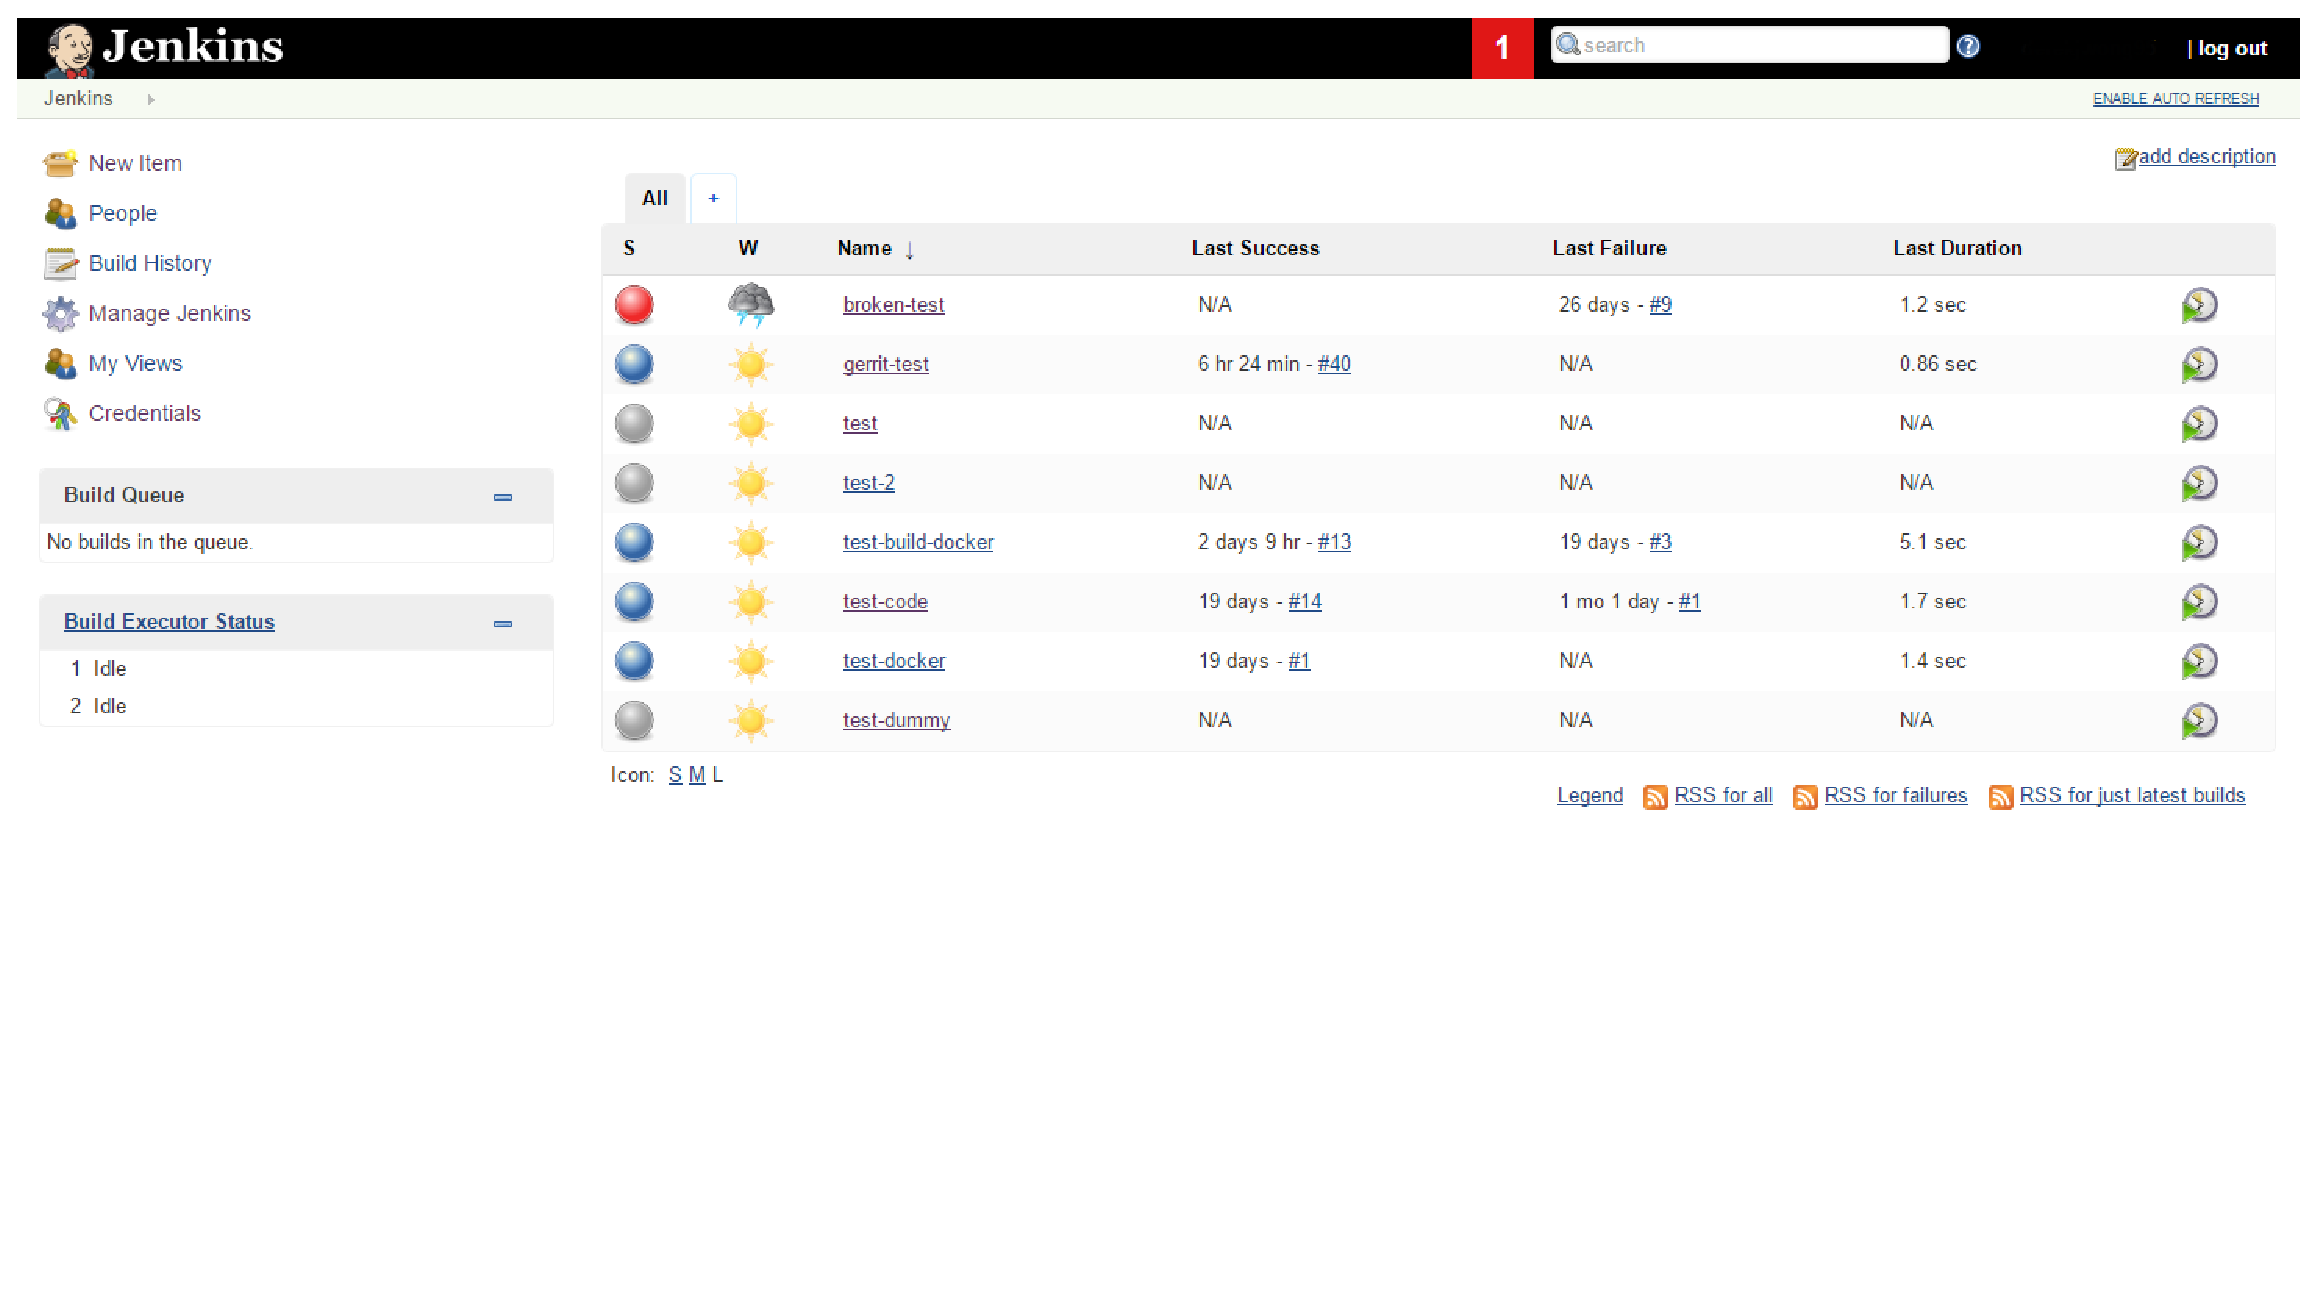
\includegraphics[width=\textwidth]{images/jenkins.eps}
  \caption{Jenkins Interface}
\end{figure}
\subsection{Configuration}

You should now be able to login to the Jenkins interface and configure the OpenStack Cloud Plugin.
Go to Manage Jenkins $\rightarrow$ Configure System. You can also label your Docker Image(s) and Build VMs so that you can specify the specific platform for individual builds.
\subsection{Workflow}
\begin{figure}[H]
  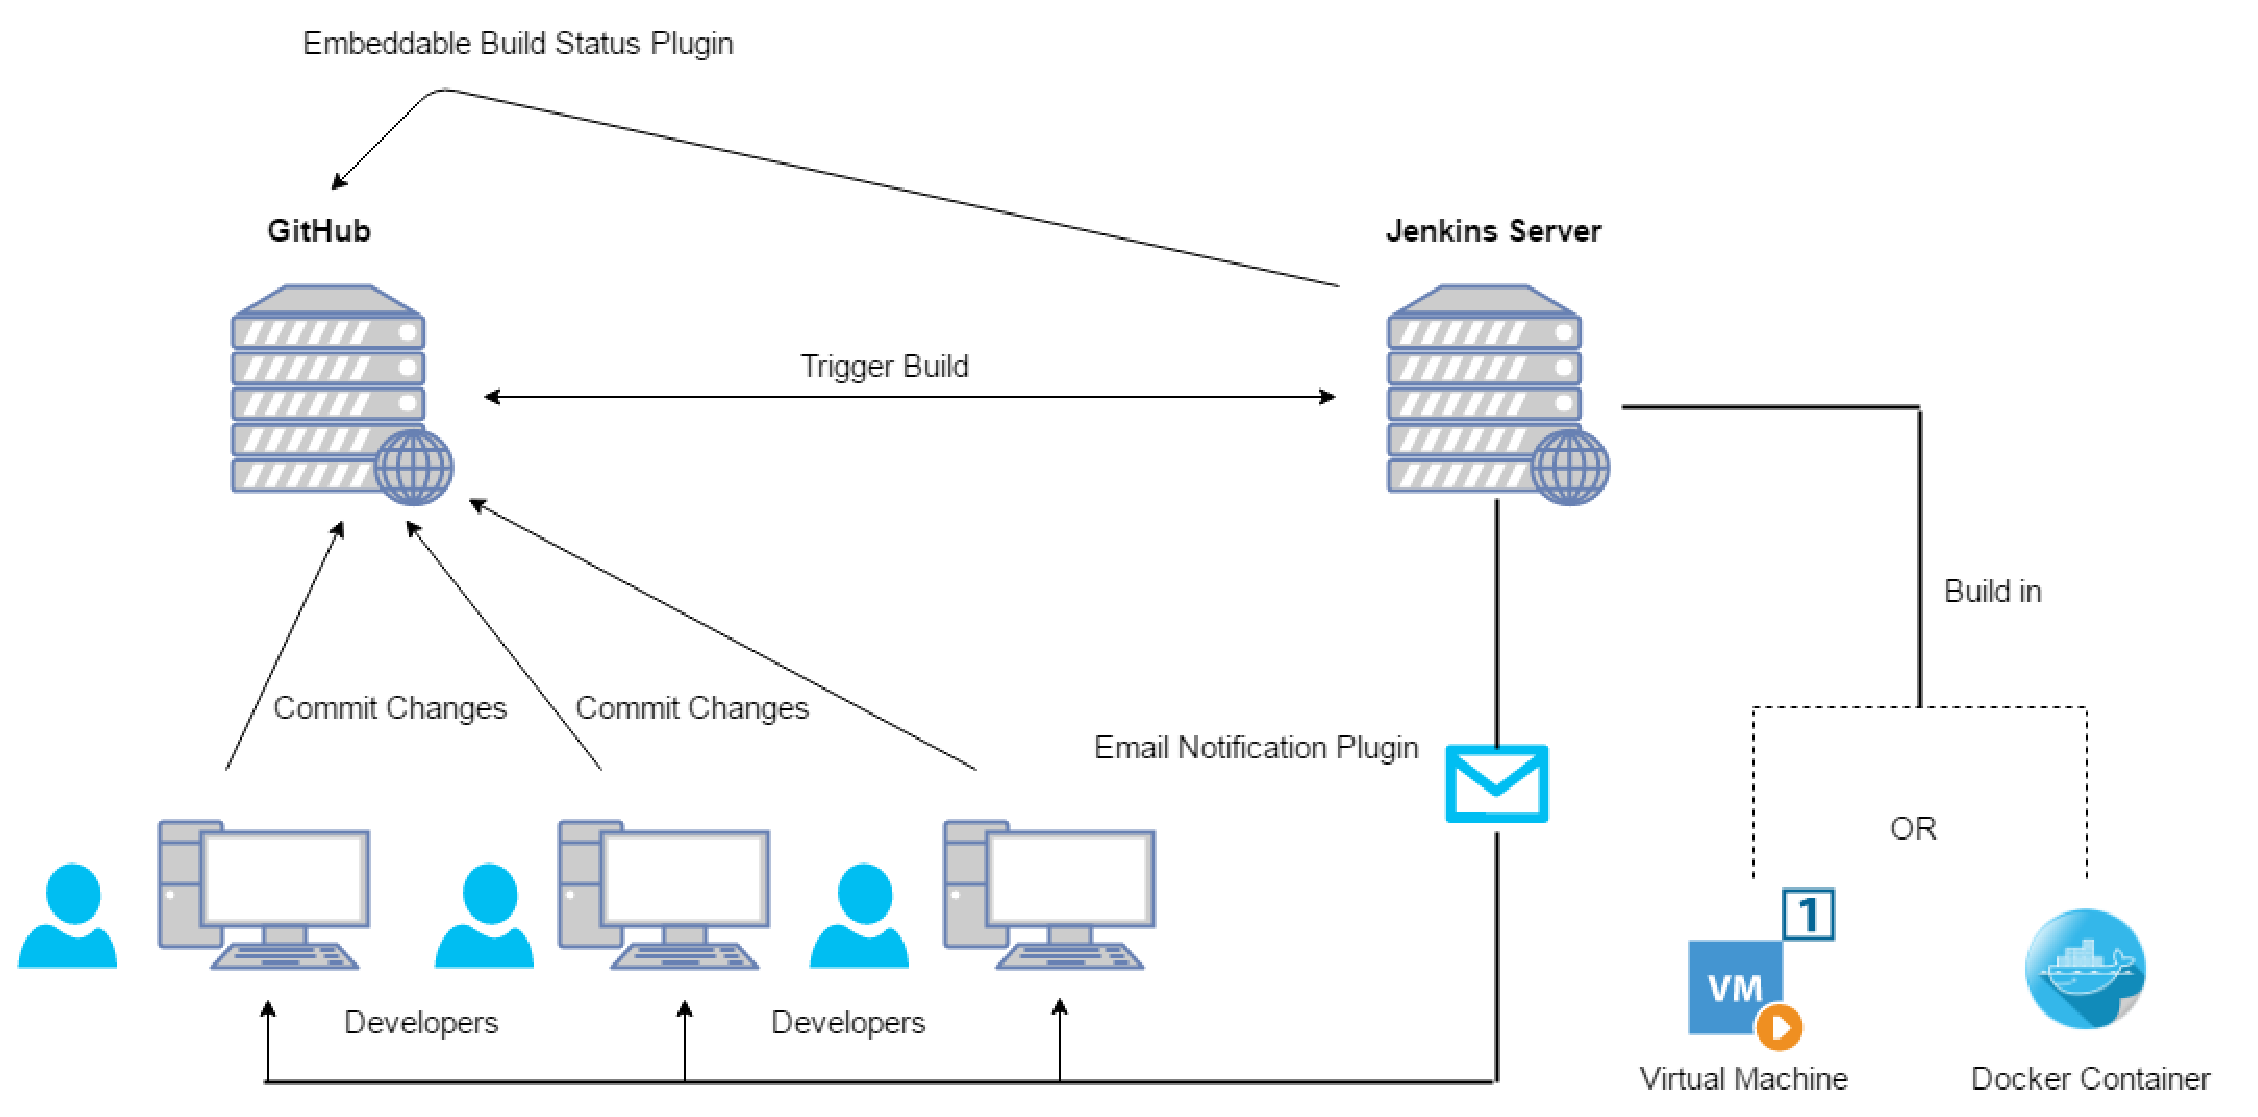
\includegraphics[width=\textwidth]{images/workflow.eps}
  \caption{POWER8 CI Workflow Diagram}
\end{figure}
\section{Learning New Technologies}
In learning new technologies we primarily relied upon web resources. For our main technologies of Jenkins, OpenStack, Docker, and Ansible
we used the documentation on their main web pages.
\begin{itemize}
  \item https://jenkins.io/doc/
  \item https://docs.openstack.org/
  \item http://docs.ansible.com/
  \item https://docs.docker.com/
\end{itemize}

In addition, our project relied heavily on various Jenkins plugins and their documentation.
\begin{itemize}
  \item https://wiki.jenkins-ci.org/display/JENKINS/Openstack+Cloud+Plugin
  \item https://wiki.jenkins-ci.org/display/JENKINS/CloudBees+Docker+Build+and+Publish+plugin
  \item https://wiki.jenkins-ci.org/display/JENKINS/Docker+Plugin
  \item https://wiki.jenkins-ci.org/display/JENKINS/Job+Restrictions+Plugin
  \item https://wiki.jenkins-ci.org/display/JENKINS/Embeddable+Build+Status+Plugin
  \item https://wiki.jenkins-ci.org/display/JENKINS/Email-ext+plugin
  \item https://wiki.jenkins-ci.org/display/JENKINS/GitHub+OAuth+Plugin
  \item https://wiki.jenkins-ci.org/display/JENKINS/Build+Monitor+Plugin
\end{itemize}

We also found Stack Exchange to be useful for finding solutions to errors that we encountered.
\begin{itemize}
  \item https://stackexchange.com/
\end{itemize}

When configuring Jenkins to run behind Apache, both the Apache documenation and the Jenkins wiki were useful.
\begin{itemize}
  \item https://httpd.apache.org/docs/
  \item https://wiki.jenkins-ci.org/display/JENKINS/Running+Jenkins+behind+Apache
\end{itemize}

In addition to these online resources, we also were able to speak to people at IBM such as our client Gerrit Huizenga
and Amit Ghatwal who assisted with the Docker configuration and with testing. We also had help from the Open Source
Lab where the project is hosted. The OSL Director Lance Albertson gave us feedback on the use of OpenStack, and Ken
Lett, the Senior Software Engineer, assisted with our understanding of Ansible.

\section{What We Learned From Capstone}
\subsection{Leon Leighton}
Going through this Capstone project has taught me quite a few things.
On the technical side, I learned about setting up services in a cloud environment and gained at least a beginners
understanding of Ansible. I also learned a great deal about configuring Jenkins. 

However, most of what I learned was not technical. 
I have learned a great deal about the need to understand the strengths and weaknesses of ones teammates 
and the importance of dividing up tasks with those strengths and weaknesses in mind. 
I have also learned how absolutely vital good communication is both within a project and with a client. 
Scheduling is also something that can be difficult, particularly when everyone has different schedules, but
I have learned that it is important to get scheduling problems resolved quickly in order to prevent delays
in working on a project.

If I could do it all over I would focus on making better use of the resources available to me.
As a student it is sometimes useful to struggle alone to understand a concept or solve a problem.
But as a member of a team trying to accomplish a goal it is better to utilize every resource available to 
meet the goal in a timely manner.
I would also try to divide up tasks and responsiblities in such a way that one person does not frequently 
block others from getting their work done. 


\subsection{Thomas Olson}
I didn't learn a lot of technical information. Some stuff about Jenkins, some about Ansible and some about OpenStack.
However, I did learn a good amount of non-technical information. In particular, how to communicate more effectively and
the importance of communicating often. I found out that project work can be fairly demanding and very stressful,
especially when there's a large amount of documentation needed and tight deadlines that must be met. I saw first-hand
how much more effective a team is when the members get together and work with one another instead of trying to work
on their own.

There are a few things I would do differently if I were to do this project all over again:

The first, by far, is to disregard being told to do development in Winter term and just start it in Fall term. The fact
of the matter is that our client wanted us to do Agile, and Agile requires rapid prototyping instead of big design
up-front. Without being able to effectively test our ideas and present prototypes until Winter term, but still having
to do our documentation in an Agile-esque way, we really didn't have a firm sense of what our design was until halfway
through Winter term, setting us back a fair bit behind schedule. By the time Fall term was over, we had essentially
wasted our and the client's time trying to do Agile development without actually doing the parts that make Agile
effective.

The second thing I'd do differently is try and organize regular times for the team to meet together for working. In one
four-to-six-hour session as a group, we'd get more done than we would in two or three weeks combined. We also would run
into problems when working apart that we wouldn't communicate effectively with each other and oftentimes failed to
leverage each team member's individual strengths to their fullest.

Third, I would try to have the work distributed more evenly. One of the issues with this project was how it had a really
bad positive feedback loop that encouraged one person to do far more work than anyone else. The inter-connectedness of
all the parts of the project combined with the steep learning curve of Ansible to put us in a situation where once one
person has a firm grasp of part of the project, it was a lot simpler to just have them do most of the work instead of
trying to get every group member on equal footing regarding the nitty-gritty of the project. This is incredibly unfair
to that one person and I would try to prevent that from occurring again.

Finally, the last thing I would do differently is engage more often with the client. On some level, we did a good job
squandering the help IBM offered us by not requesting help when we needed it and by trying to solve problems on our own
instead of asking IBM questions.

\subsection{Derek Wong}
Throughout this project I've learned many technical and non-technical skills.
This project introduced me to continuous integration which many software development team uses.
Our project was to create a continuous integration for IBM's POWER8 machine and the technologies used were:
OpenStack, Jenkins, and Ansible. I learned a little about OpenStack and its ability to create VMs and Docker Containers.
As for Jenkins, I already had prior knowledge of this technology from an internship I had before.
For Ansible, I learned about the "Playbook" which was what we used to install our system and
all the add-ons we had and the configurations as well.
From working on this project, I learned that having a well defined workflow is really important.
It provides a structure of how task can be accomplished and it makes it easier to divide work amongst team members.
Sharing schedule with team members and having a deadline for each task or just milestone in 
general is really useful in project management.
I learned that working in teams, communication is the most important.
It is really hard to work on a team project if we can't communicate with our group members or what task is each person is working on.
If I could do this project all over again, I would begin the project more early and have a well defined workflow.
In the beginning, I was confused and I didn't know where to start and had to rely on my group members to guide me.
I would look into my project earlier and try to do more research and learn more about it so I 
had a good grasp of what I needed to do when our group began to work on the project.

\clearpage
\bibliographystyle{IEEEtran}
\bibliography{final}
\clearpage

\section{Appendix 1}

\begin{lstlisting}[caption=Ansible Host file]
[jenkins]
power-ci.osuosl.org ansible_python_interpreter=/usr/bin/python2.7
\end{lstlisting}

\begin{lstlisting}[caption=Ansible Playbook]
- name: Install and configure Jenkins
  hosts: jenkins
  roles:
    - geerlingguy.jenkins
    - jenkins
    - web
  remote_user: ubuntu
  become: yes
  vars_files:
- group_vars/jenkins
\end{lstlisting}


\begin{lstlisting}[caption=Playbook Variables]
jenkins_hostname: power-ci.osuosl.org
\end{lstlisting}

\begin{lstlisting}[caption=Jenkins Task]
- name: Include Secret Variables
  include_vars: secret.yml

- name: Create Plugin Directory
  file: path=/var/lib/jenkins/plugins state=directory

- name: Install Build Monitor Plugin
  jenkins_plugin:
    name: build-monitor-plugin
    params: "{{ my_jenkins_params }}"

- name: Install Matrix Authorization Plugin
  jenkins_plugin:
    name: matrix-auth
    params: "{{ my_jenkins_params }}"

- name: Install Docker-Build-Publish Plugin
  jenkins_plugin:
    name: docker-build-publish
    params: "{{ my_jenkins_params }}"

- name: Install Docker Plugin
  jenkins_plugin:
    name: docker-plugin
    params: "{{ my_jenkins_params }}"

- name: Install Email Notification Plugin
  jenkins_plugin:
    name: emailext-template
    params: "{{ my_jenkins_params }}"

- name: Install Embeddable Build Status Plugin
  jenkins_plugin:
    name: embeddable-build-status 
    params: "{{ my_jenkins_params }}"

- name: Install GitHub Branch Source Plugin
  jenkins_plugin:
    name: github-branch-source
    params: "{{ my_jenkins_params }}"


- name: Install Multibranch Plugin
  jenkins_plugin:
    name: workflow-multibranch
    params: "{{ my_jenkins_params }}"


- name: Install GitHub Oauth Plugin
  jenkins_plugin:
    name: github-oauth
    params: "{{ my_jenkins_params }}"

- name: Install GitHub Plugin
  jenkins_plugin:
    name: github 
    params: "{{ my_jenkins_params }}"

- name: Install Job Restrictions Plugin
  jenkins_plugin:
    name: job-restrictions 
    params: "{{ my_jenkins_params }}"

- name: Install OpenStack Cloud Plugin
  jenkins_plugin:
    name: openstack-cloud 
    params: "{{ my_jenkins_params }}"

- name: Configure GitHub Oauth Plugin in Jenkins
  template: >
    src=./roles/jenkins/templates/config-oauth.groovy.j2
    dest=/var/lib/jenkins/init.groovy.d/config-oauth.groovy
    owner=jenkins
    group=jenkins

- name: Configure Docker in Jenkins
  template: >
    src=./roles/jenkins/templates/config-docker.groovy.j2
    dest=/var/lib/jenkins/init.groovy.d/config-docker.groovy
    owner=jenkins
    group=jenkins

- name: Install Email config
  copy: src=hudson.tasks.Mailer.xml dest=/var/lib/jenkins/ mode=0644

- name: Restart Jenkins 
  service:
    name: jenkins
    state: restarted
\end{lstlisting}

\begin{lstlisting}[caption=Template for configuring authentication]
import hudson.security.*
import jenkins.model.*
import org.jenkinsci.plugins.GithubAuthorizationStrategy
import hudson.security.AuthorizationStrategy
import hudson.security.SecurityRealm
import org.jenkinsci.plugins.GithubSecurityRealm
import hudson.security.ProjectMatrixAuthorizationStrategy
import hudson.security.csrf.DefaultCrumbIssuer

Jenkins.instance.crumbIssuer = new DefaultCrumbIssuer(true)

// Authenticatin
String githubWebUri = 'https://github.com'
String githubApiUri = 'https://api.github.com'
String clientID = '{{ oauth.clientid }}'
String clientSecret = '{{ oauth.clientsecret }}'
String oauthScopes = 'read:org'
SecurityRealm github_realm = new GithubSecurityRealm(githubWebUri, githubApiUri, clientID, clientSecret, oauthScopes)
//check for equality, no need to modify the runtime if no settings changed
if(!github_realm.equals(Jenkins.instance.getSecurityRealm())) {
    Jenkins.instance.setSecurityRealm(github_realm)
    Jenkins.instance.save()
}

// Authorization
class BuildPermission {
  static buildNewAccessList(userOrGroup, permissions) {
    def newPermissionsMap = [:]
    permissions.each {
      newPermissionsMap.put(Permission.fromId(it), userOrGroup)
    }
    return newPermissionsMap
  }
}

auth_strategy = new hudson.security.ProjectMatrixAuthorizationStrategy()

authenticatedPermissions = [ "hudson.model.Hudson.Read" ]
authenticated = BuildPermission.buildNewAccessList("authenticated", authenticatedPermissions)
authenticated.each { p, u -> auth_strategy.add(p, u) }

adminPermissions = [
	"com.cloudbees.plugins.credentials.CredentialsProvider.Create",
	"com.cloudbees.plugins.credentials.CredentialsProvider.Delete",
	"com.cloudbees.plugins.credentials.CredentialsProvider.ManageDomains",
	"com.cloudbees.plugins.credentials.CredentialsProvider.Update",
	"com.cloudbees.plugins.credentials.CredentialsProvider.View",
	"hudson.model.Computer.Build",
	"hudson.model.Computer.Configure",
	"hudson.model.Computer.Connect",
	"hudson.model.Computer.Create",
	"hudson.model.Computer.Delete",
	"hudson.model.Computer.Disconnect",
//	"hudson.model.Computer.Provision",
	"hudson.model.Hudson.Administer",
	"hudson.model.Hudson.Read",
	"hudson.model.Item.Build",
	"hudson.model.Item.Cancel",
	"hudson.model.Item.Configure",
	"hudson.model.Item.Create",
	"hudson.model.Item.Delete",
	"hudson.model.Item.Discover",
	"hudson.model.Item.Read",
	"hudson.model.Item.ViewStatus",
	"hudson.model.Item.Workspace",
	"hudson.model.Run.Delete",
	"hudson.model.Run.Update",
	"hudson.model.View.Configure",
	"hudson.model.View.Create",
	"hudson.model.View.Delete",
	"hudson.model.View.Read"
]

admin = BuildPermission.buildNewAccessList("{{ aduser }}", adminPermissions)
admin.each { p, u -> auth_strategy.add(p, u) }


userPermissions = [
	"hudson.model.Item.Build",
	"hudson.model.Item.Cancel",
	"hudson.model.Item.Configure",
	"hudson.model.Item.Create",
	"hudson.model.Item.Delete",
	"hudson.model.Item.Discover",
	"hudson.model.Item.Read",
	"hudson.model.Item.ViewStatus",
	"hudson.model.Item.Workspace"
]

user = BuildPermission.buildNewAccessList("{{ nuser }}", userPermissions)
user.each { p, u -> auth_strategy.add(p, u) }


//check for equality, no need to modify the runtime if no settings changed
if(!auth_strategy.equals(Jenkins.instance.getAuthorizationStrategy())) {
    Jenkins.instance.setAuthorizationStrategy(auth_strategy)
    Jenkins.instance.save()
}
\end{lstlisting}

\begin{lstlisting}[caption=]

\end{lstlisting}

\begin{lstlisting}[caption=]

\end{lstlisting}


\end{document}
